\documentclass[tikz]{standalone}
% \usepackage{tikz} % already loaded by the documentclass


\begin{document}
%%| caption: Triangle Graph - Our working example with vertices 0, 1, 2

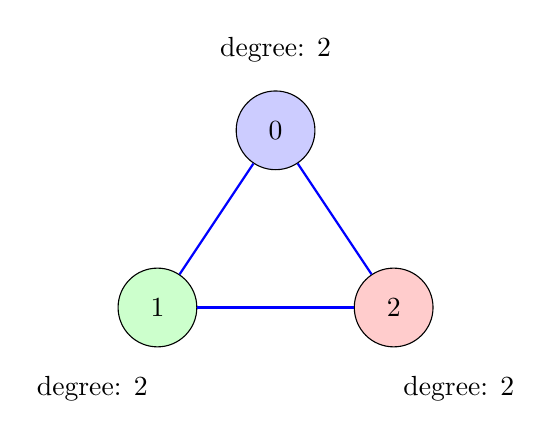
\begin{tikzpicture}[scale=1.5]
  % Define vertices
  \node[circle, draw, fill=blue!20, minimum size=1cm] (0) at (0,1.5) {0};
  \node[circle, draw, fill=green!20, minimum size=1cm] (1) at (-1,0) {1};
  \node[circle, draw, fill=red!20, minimum size=1cm] (2) at (1,0) {2};

  % Draw edges
  \draw[thick, blue] (0) -- (1);
  \draw[thick, blue] (1) -- (2);
  \draw[thick, blue] (2) -- (0);

  % Add degree labels
  \node[above] at (0,2) {degree: 2};
  \node[below left] at (-1,-0.5) {degree: 2};
  \node[below right] at (1,-0.5) {degree: 2};
\end{tikzpicture}
\end{document}
      